\documentclass{article}
\usepackage{graphicx} % Required for inserting images
\usepackage{float}

\title{BPC Gripper Assembly Demo}
\author{}
\date{September 2024}

\begin{document}

\maketitle

\section{Introduction}
In this guide, you’ll learn how to build your very own Gripper! We’ll take it step by step, showing you how to put together all the parts to make the Gripper work. You’ll start by gathering the pieces you need, then work on building the base, attaching the fingers, and connecting the electronics. Don’t worry if you’ve never done something like this before – just follow along, and by the end, you’ll have a Gripper you built yourself!

\section{Required Parts}
\begin{table}[H]
    \centering
    \begin{tabular}{|c|l|c|}
        \hline
        \textbf{Number} & \textbf{Component} & \textbf{Quantity} \\
        \hline
        1  & Base Plate                & 1  \\
        2  & Top Plate                 & 1  \\
        3  & Plate Connector           & 4  \\
        4  & Servo                     & 4  \\
        5  & Encoder                   & 4  \\
        6  & Silicone Finger           & 4  \\
        7  & Ultrasonic Distance Sensor & 1  \\
        8  & Red Push Button           & 1  \\
        9  & Voltage Regulator         & 1  \\
        10 & Metro Mini V2             & 1  \\
        11 & MPR121                    & 1  \\
        12 & Finger Mount Base         & 4  \\
        13 & Finger Mount Top          & 4  \\
        14 & Finger Mount Screw        & 4  \\
        15 & Servo Standoff Clips      & 8  \\
        16 & Spool (Magnet) Base       & 4  \\
        17 & Spool Top                 & 4  \\
        18 & Encoder Disc              & 4  \\
        19 & Encoder Housing           & 4  \\
        20 & Servo Mount               & 4  \\
        21 & Encoder Disc Connector    & 4  \\
        22 & PCB                       & 1  \\
        23 & Power Adapter             & 1  \\
        24 & M3-0.5 Nut                & 8  \\
        25 & 4-40 x 3/8 Flat Head Screw & 8  \\
        26 & M3-05 6mm Standoff        & 4  \\
        27 & M3 x 6mm Hex Screw        & 4  \\
        28 & M 2.5x10 Hex Screw        & 8  \\
        29 & Encoder Jumper Cables     & 8  \\
        30 & Distance Sensor Standoffs & 2  \\
        \hline
    \end{tabular}
    \caption{Component List: Note that the color of the components may not line up with what you have in your kit}
\end{table}

\begin{figure}[H]
    \centering
    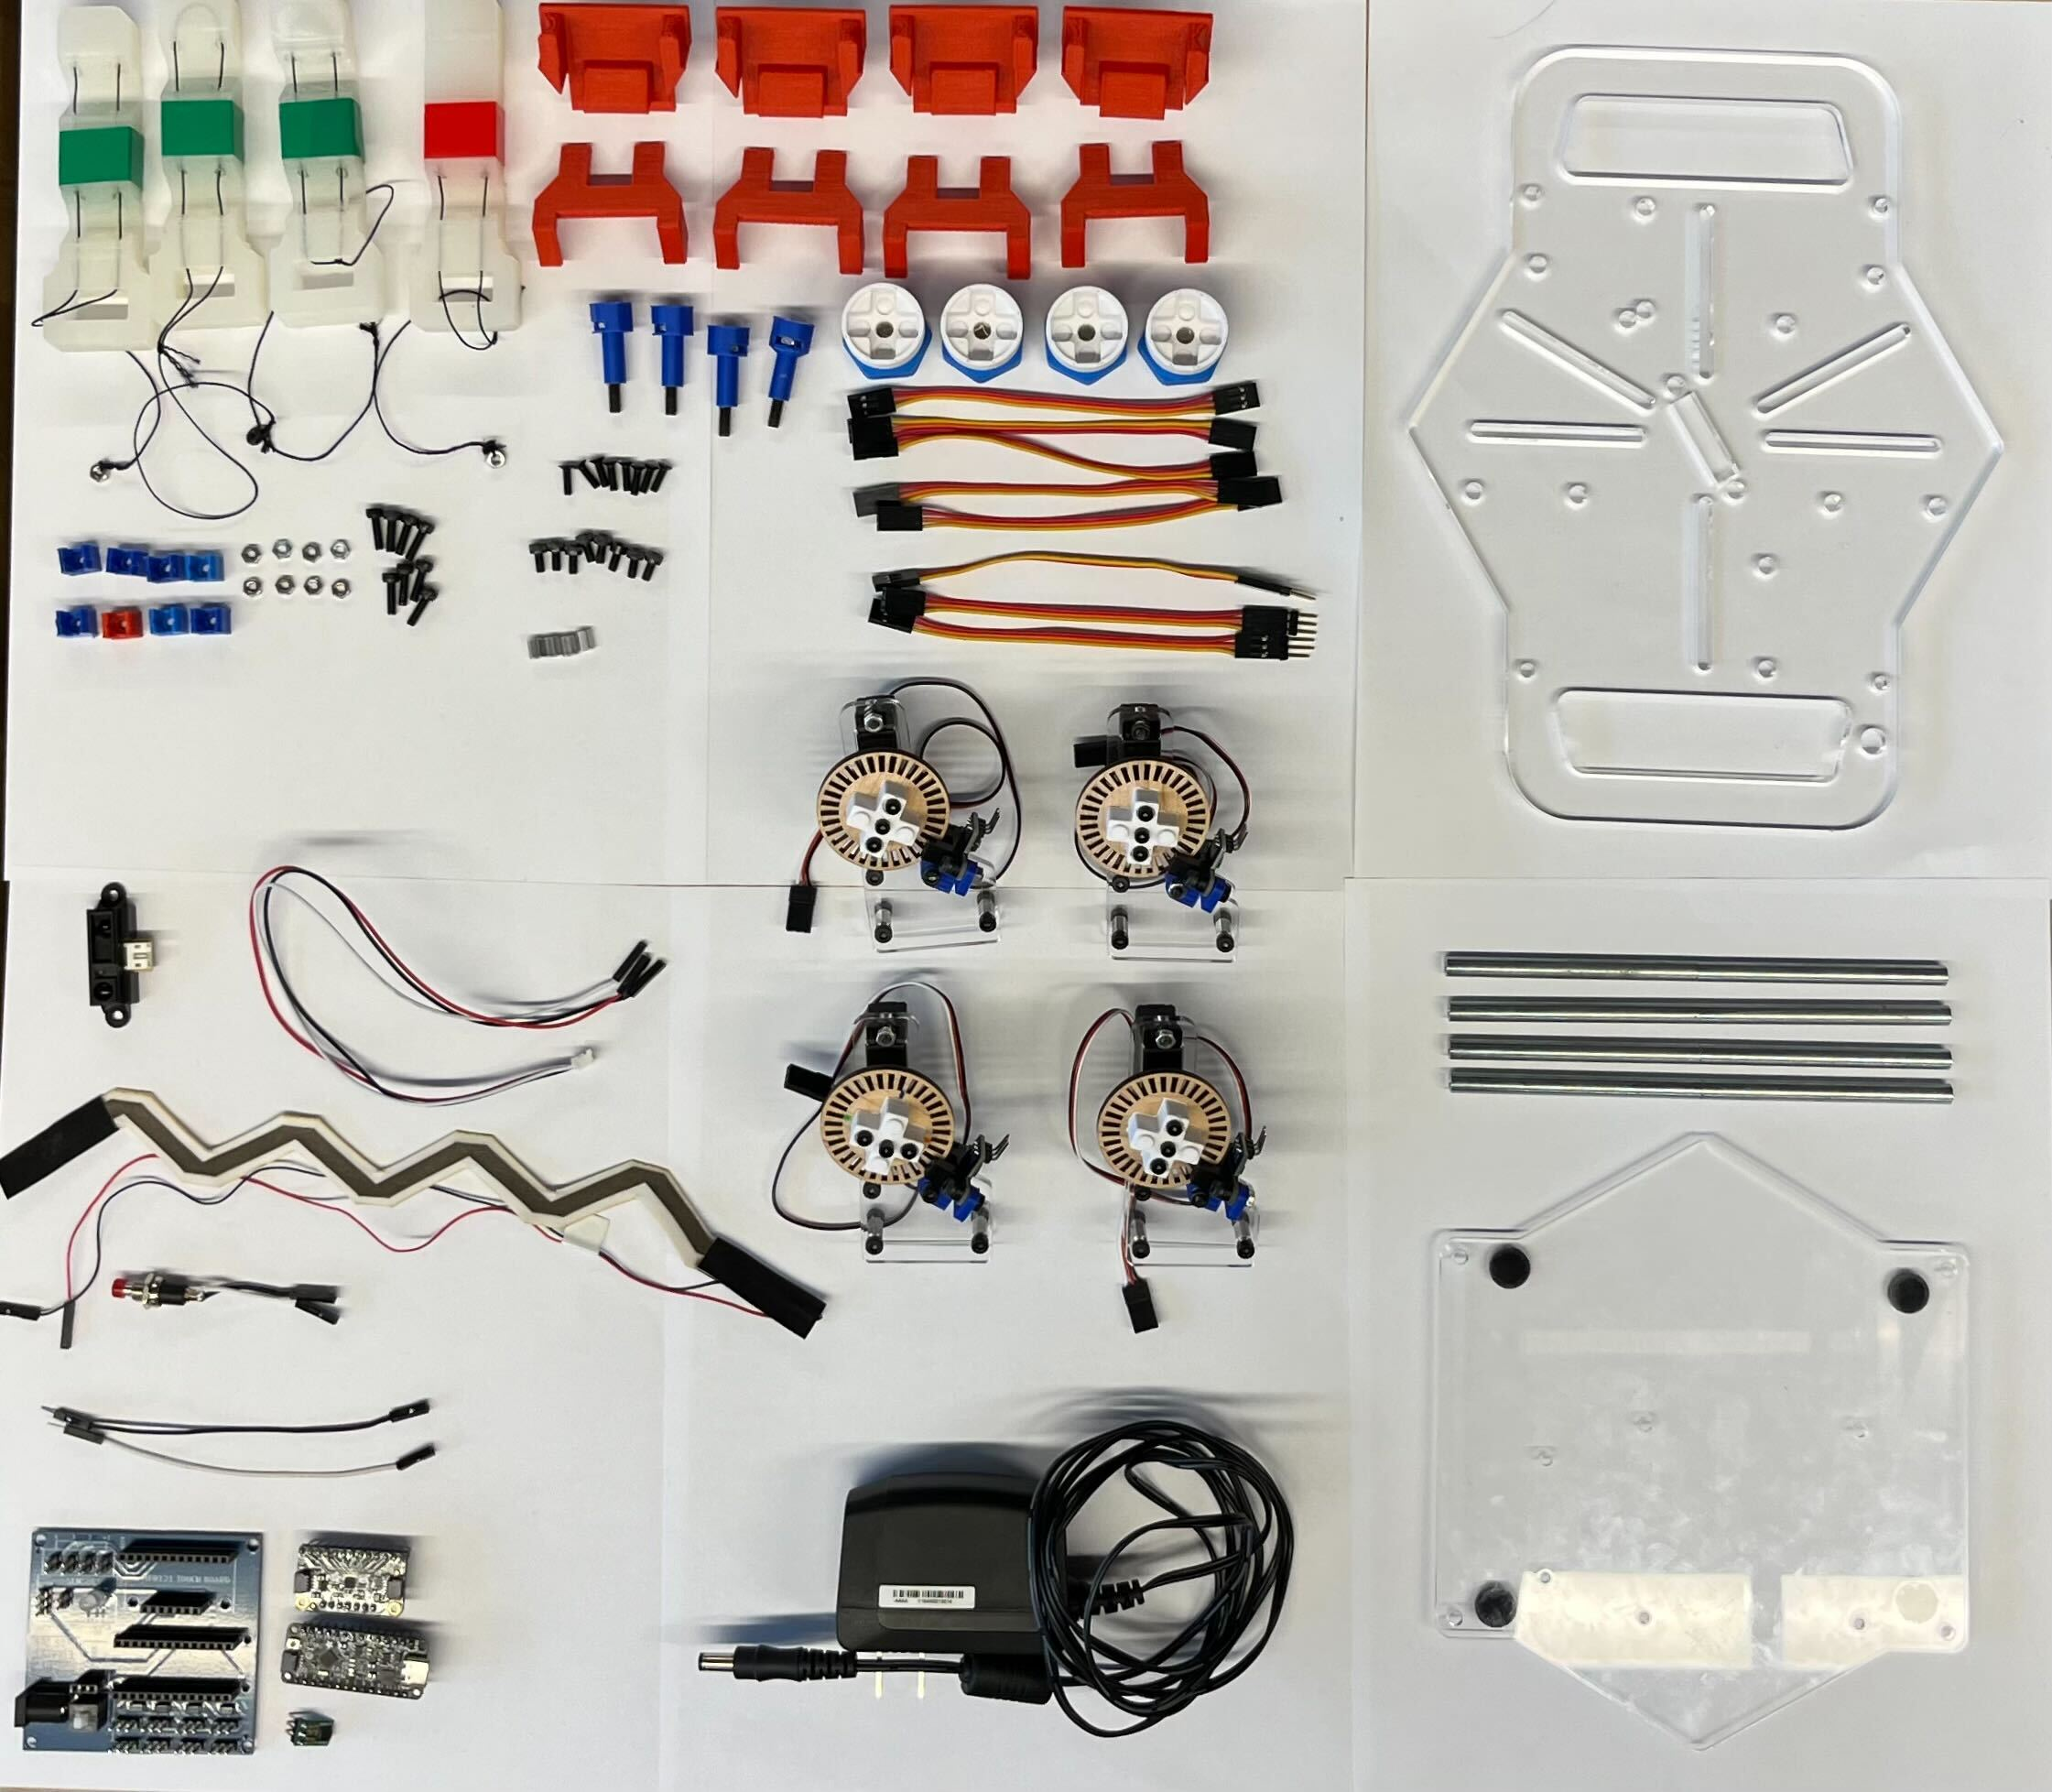
\includegraphics[scale = .15]{PCBImages/parts_overhead.jpg}
    \caption{All of the Components}
    \label{fig:components_image}
\end{figure}

\section{Building the Base}
\begin{figure}[H]
    \centering
    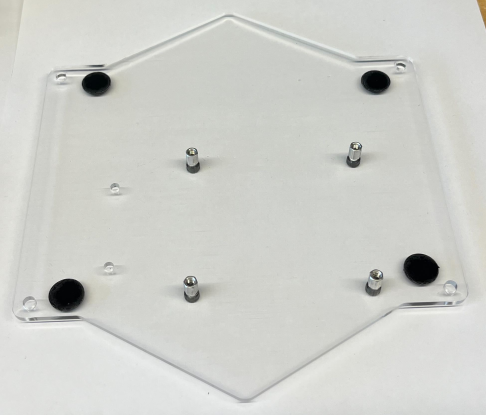
\includegraphics[width=0.5\linewidth]{PCBImages/Frame/frame_1.png}
    \caption{The Base Plate}
    \label{fig:base_plate}
\end{figure}

\subsection{Screwing in the PCB}
To begin, you'll need to set aside 4 of the M3x6mm Hex Screws. After that, place the PCB on the four standoffs that are located on the Base Plate. You'll want to make sure the corner holes on the PCB align with the screw holes on the Base Plate Standoffs. The PCB is a rectangle, so either horizontal orientation is fine. Once placed, screw in the screws for all four corners.

\begin{figure}[H]
    \centering
    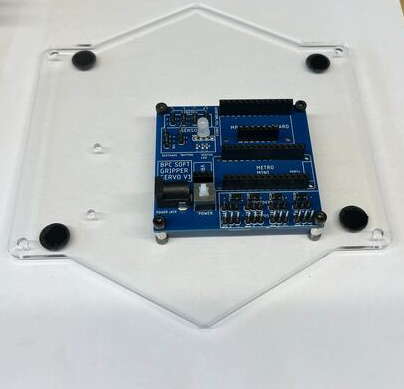
\includegraphics[width=0.5\linewidth]{PCBImages/Frame/frame_2.png}
    \caption{The Base Plate with the PCB on it}
    \label{fig:base_with_pcb}
\end{figure}

\subsection{Connecting the Base Plate to the Top Plate}
Now, you'll want to locate the 4 Plate Connectors. These are 4 Long Silver Cylindrical Rods with holes on both sides of them. First, place one of the ends over the holes located at each corner of the base plate. Once aligned, use one of the 4-40 x 3/8 Flat Head Screws to attach the Connector to the Base Plate. Repeat this for the remaining Connectors.

Once the Connectors are on the Base Plate, align the Top Plate so that the screw holes located on the corners of the Top Plate align with the holes on the Connectors. Use the remaining 4-40 x 3/8 Flat Head Screws to finish connecting the Top Plate to the Base Plate.

\begin{figure}[H]
    \centering
    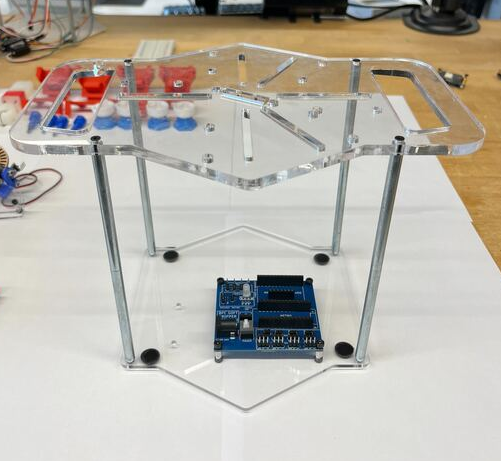
\includegraphics[width=0.5\linewidth]{PCBImages/Frame/frame_3.png}
    \caption{The Base and Top Plate Connected}
    \label{fig:base_top_connected}
\end{figure}

\subsection{Mounting the Ultrasonic Distance Sensor}
\begin{figure}[H]
    \centering
    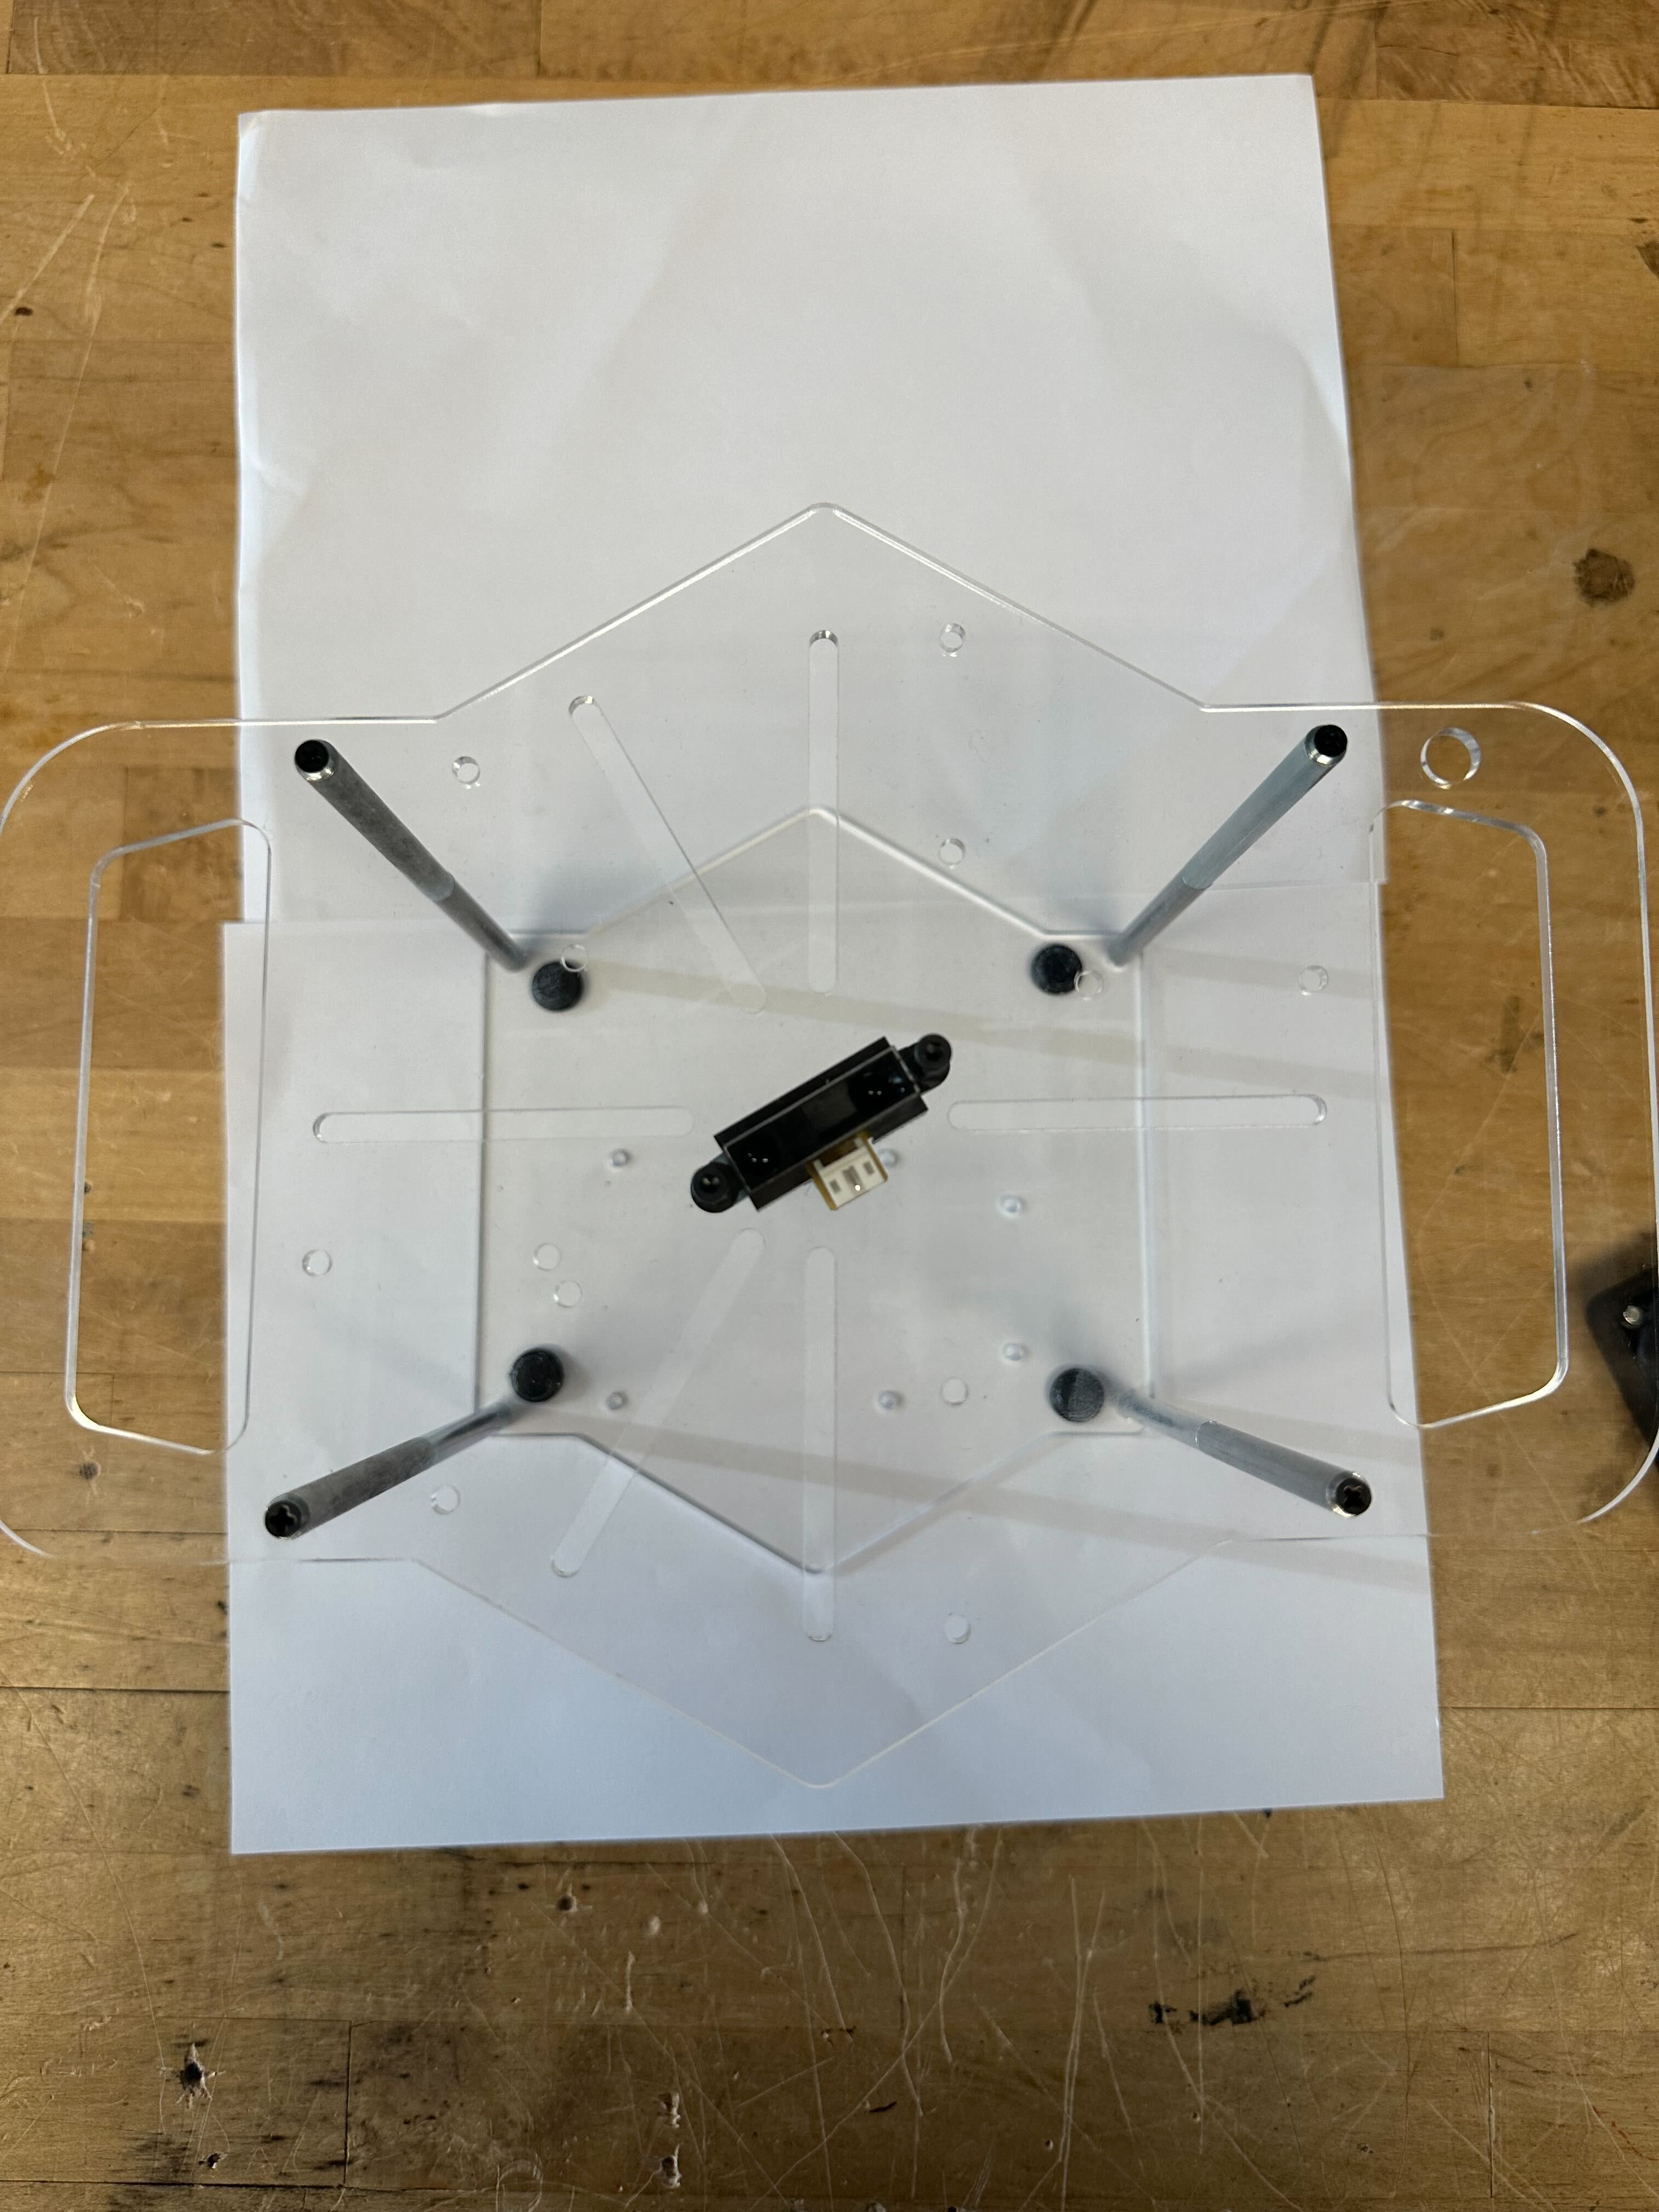
\includegraphics[width=0.5\linewidth]{PCBImages/Frame/ultrasonic-distance-on-top-plate.jpg}
    \caption{Ultrasonic Distance Sensor on the Top Plate}
    \label{fig:ultrasonic_on_top_plate}
\end{figure}

\subsection{Mounting the Red Push Button to the Top Plate}
\begin{figure}[H]
    \centering
    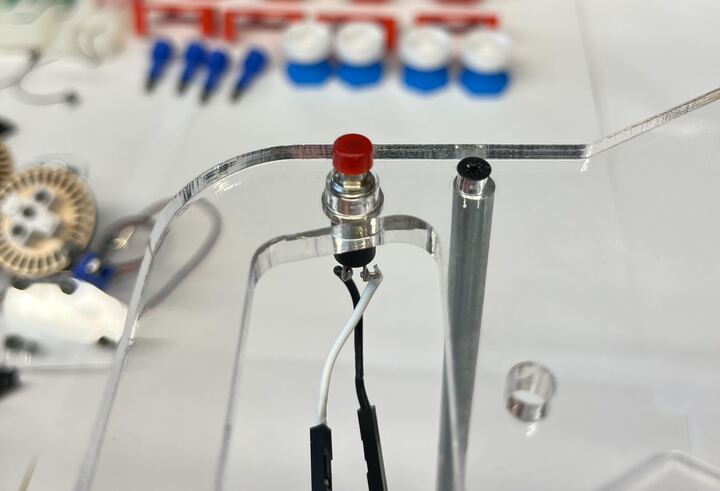
\includegraphics[width=0.5\linewidth]{PCBImages/Frame/frame_5.jpg}
    \caption{The Red Push Button on the Top Plate}
    \label{fig:red_button_on_top_plate}
\end{figure}

\section{Attaching the Fingers}
\begin{figure}[H]
    \centering
    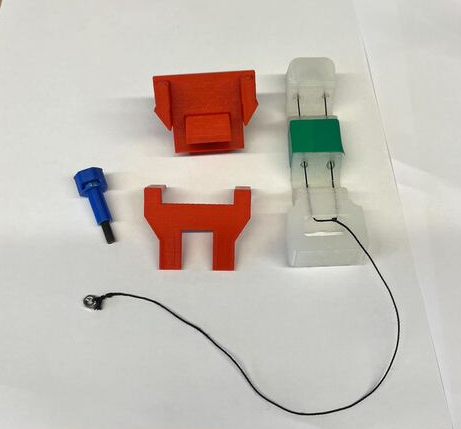
\includegraphics[width=0.5\linewidth]{PCBImages/AttachingFingers/attaching_fingers_1.png}
    \caption{The different parts of the Silicone Fingers}
    \label{fig:silicone_fingers_parts}
\end{figure}

\subsection{Assembling the Finger Mount}
\begin{figure}[H]
    \centering
    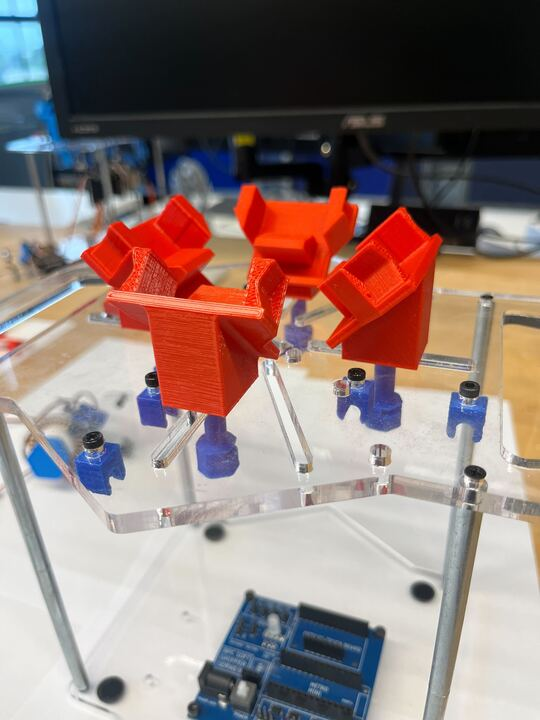
\includegraphics[width=0.5\linewidth]{PCBImages/AttachingFingers/attaching_fingers_2.jpg}
    \caption{The Finger Mounts on the Top Plate}
    \label{fig:finger_mount_top_plate}
\end{figure}

\subsection{Placing the Fingers on the Mount}
\begin{figure}[H]
    \centering
    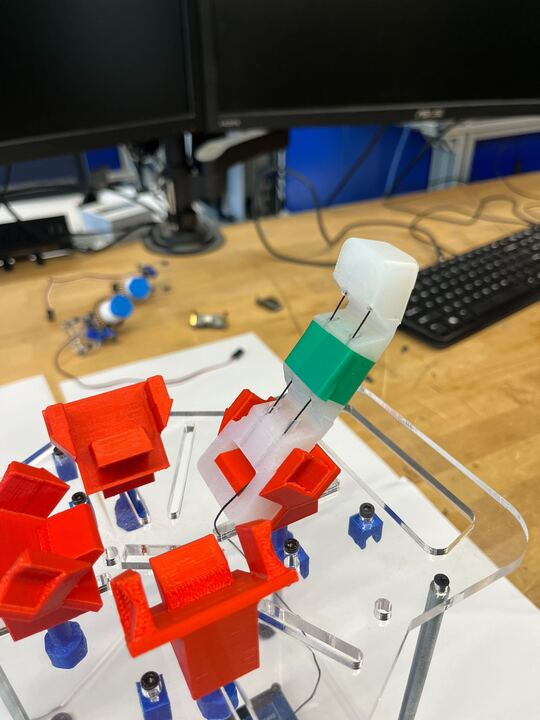
\includegraphics[width=0.5\linewidth]{PCBImages/AttachingFingers/attaching_fingers_3.jpg}
    \caption{The Finger on the Finger Mount Base}
    \label{fig:finger_on_mount_base}
\end{figure}
\begin{figure}[H]
    \centering
    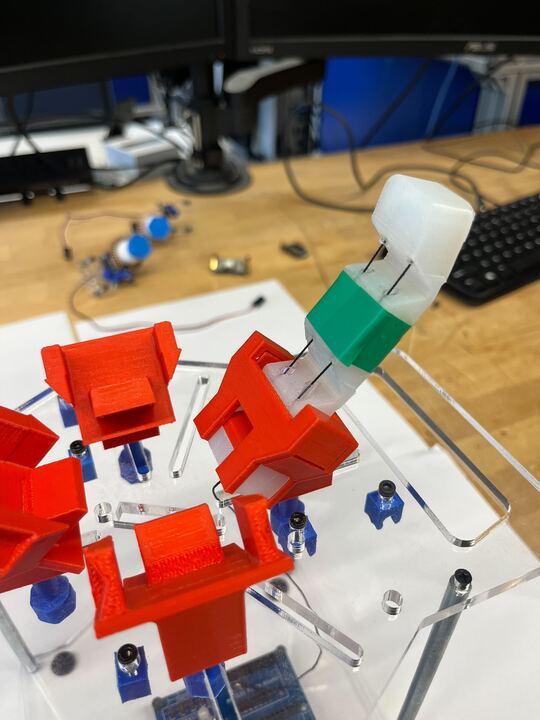
\includegraphics[width=0.5\linewidth]{PCBImages/AttachingFingers/attaching_fingers_4.jpg}
    \caption{The Finger secured to the Finger Mount Base with the Finger Mount Top}
    \label{fig:finger_on_mount_top}
\end{figure}

\begin{figure}[H]
    \centering
    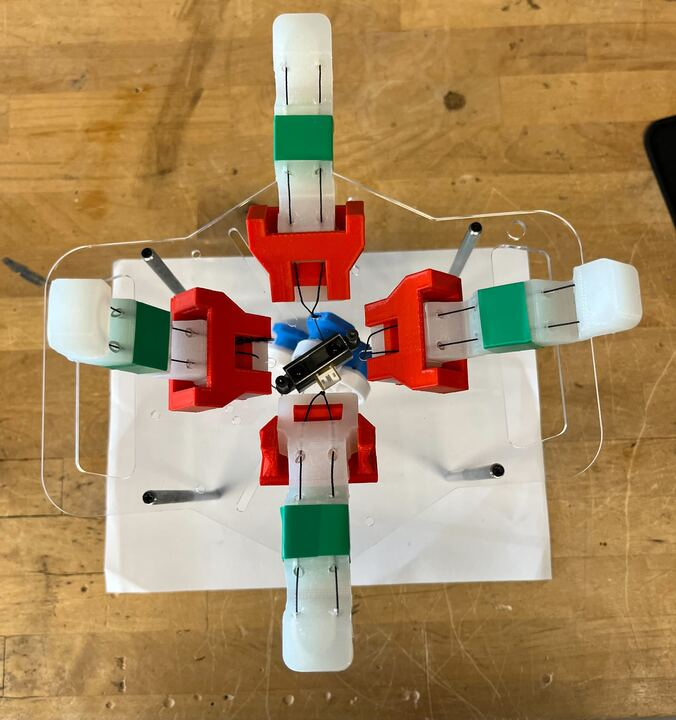
\includegraphics[width=0.5\linewidth]{PCBImages/AttachingFingers/attaching_fingers_5.jpg}
    \caption{All Fingers Mounted on the Top Plate}
    \label{fig:all_fingers_mounted}
\end{figure}

\subsection{Spooling the Finger's String on the Spool}
\begin{figure}[H]
    \centering
    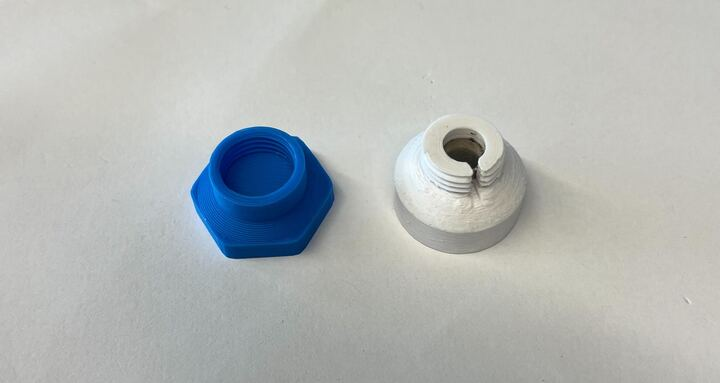
\includegraphics[width=0.5\linewidth]{PCBImages/Spools/spools_1.jpg}
    \caption{The Spool Top and the Spool (Magnet) Base}
    \label{fig:spool_top_and_base}
\end{figure}
\begin{figure}[H]
    \centering
    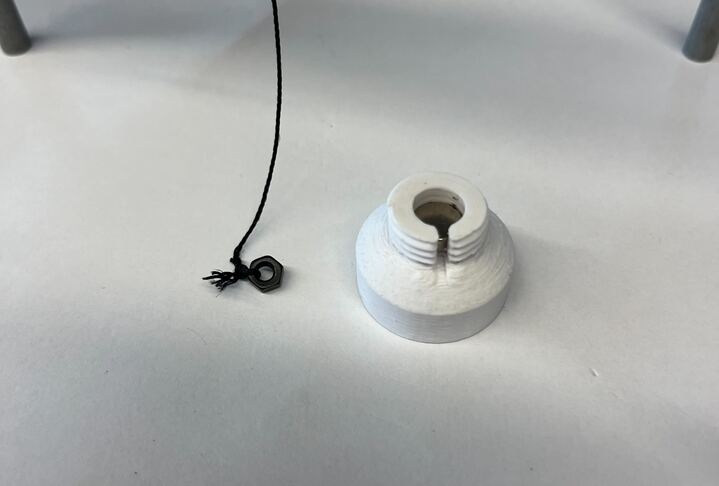
\includegraphics[width=0.5\linewidth]{PCBImages/Spools/spools_2.jpg}
    \caption{The Spool Base and the Finger Nut}
    \label{fig:spool_base_and_finger_nut}
\end{figure}
\begin{figure}[H]
    \centering
    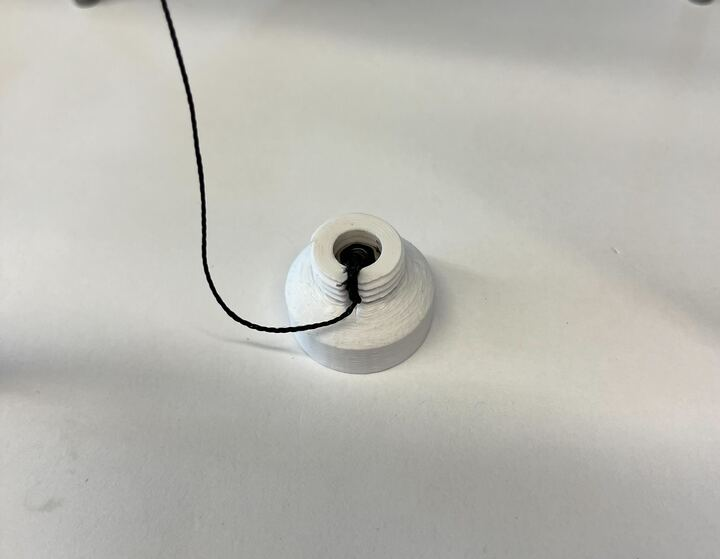
\includegraphics[width=0.5\linewidth]{PCBImages/Spools/spools_3.jpg}
    \caption{The Finger Nut attached to the Magnet of the Spool Base}
    \label{fig:finger_nut_attached}
\end{figure}
\begin{figure}[H]
    \centering
    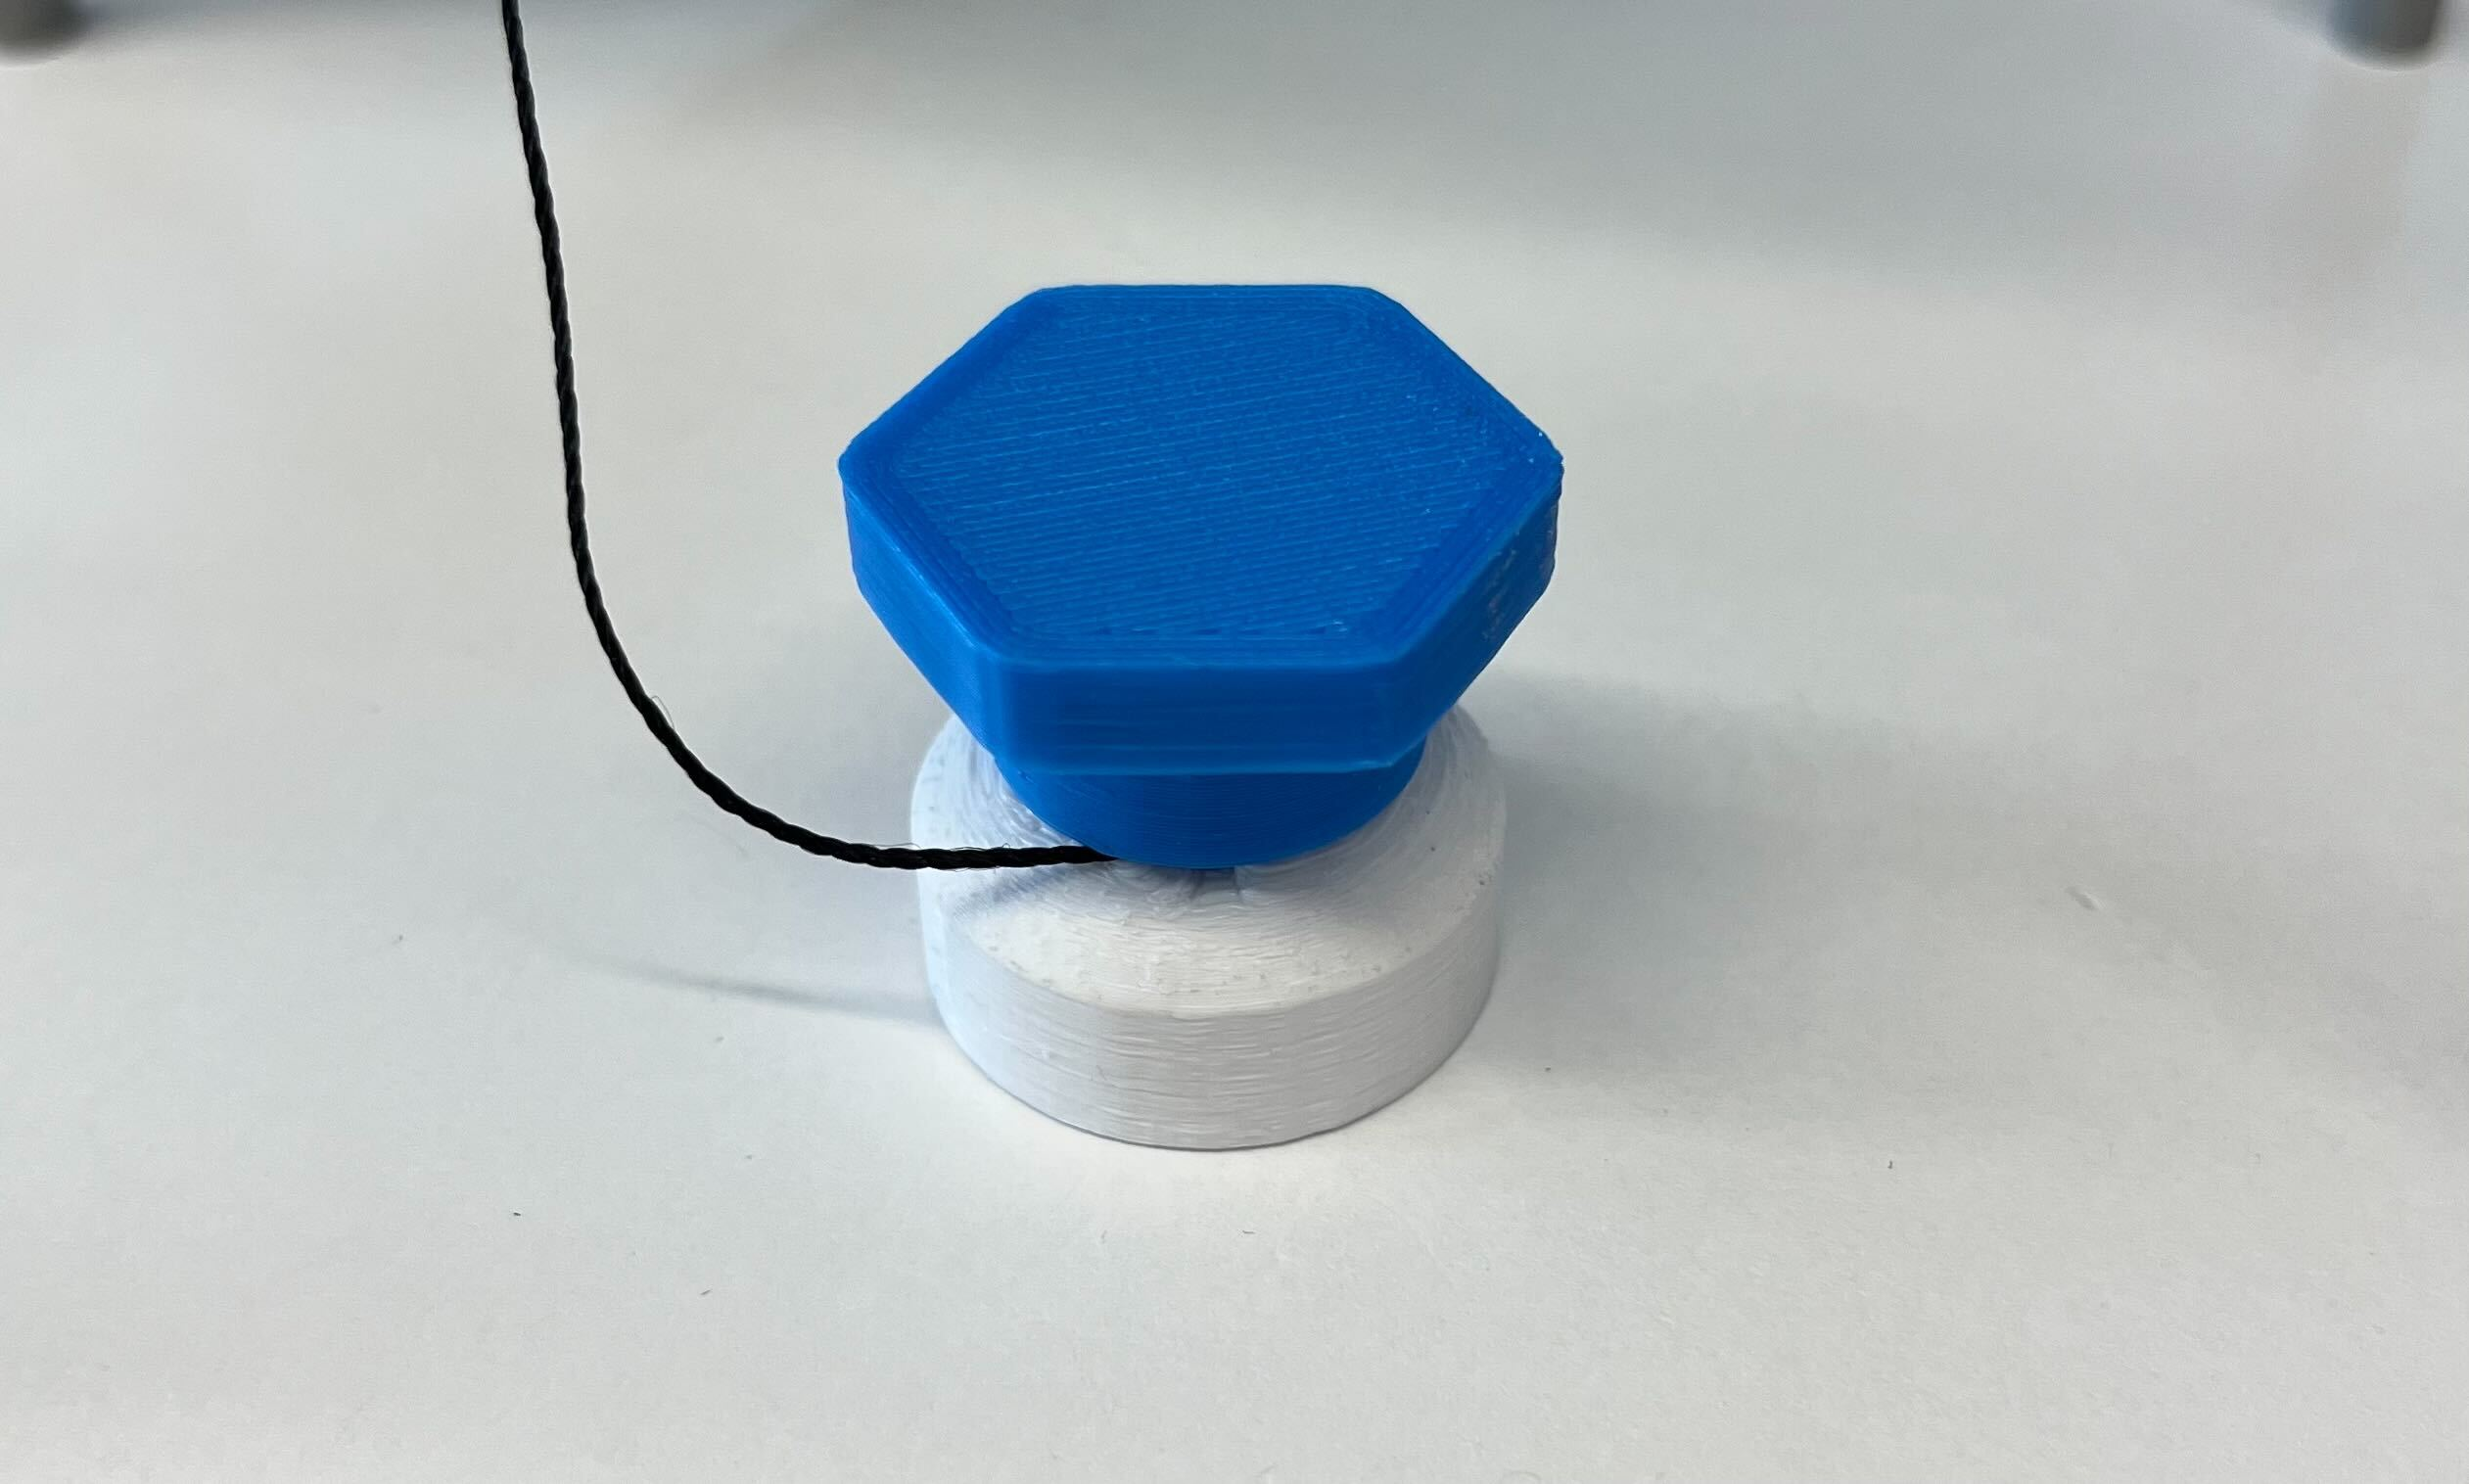
\includegraphics[width=0.5\linewidth]{PCBImages/Spools/spools_4.jpg}
    \caption{The Spool Top screwed onto the Spool Base}
    \label{fig:spool_top_screwed}
\end{figure}

\section{Servo Hardware}

\subsection{Attaching the Servo Standoff Clips}
\begin{figure}[H]
    \centering
    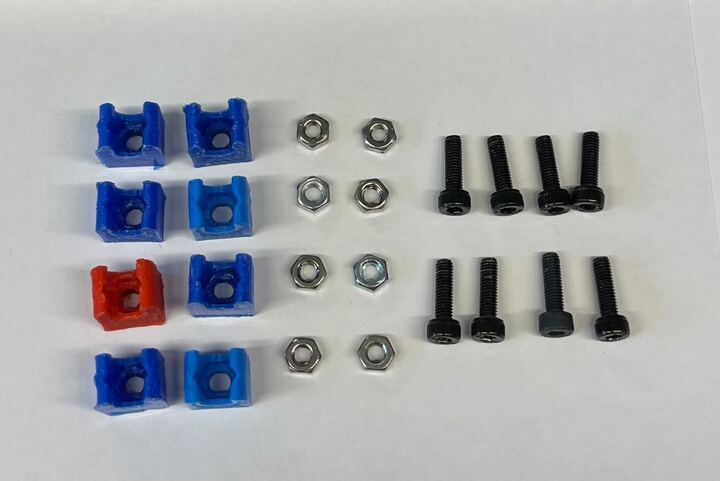
\includegraphics[width=0.5\linewidth]{PCBImages/StandoffClips/standoff_clips_1.jpg}
    \caption{The Servo Clips and their Hardware}
    \label{fig:servo_clips_hardware}
\end{figure}
\begin{figure}[H]
    \centering
    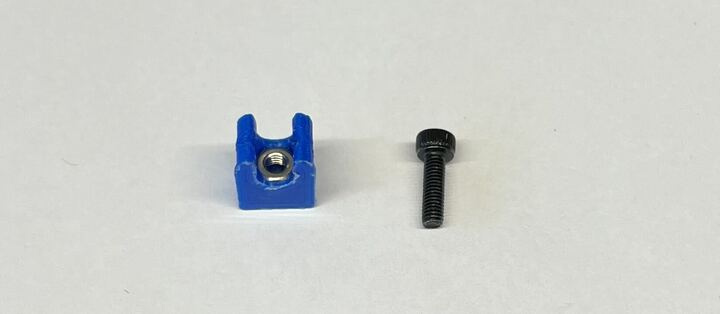
\includegraphics[width=0.5\linewidth]{PCBImages/StandoffClips/standoff_clips_3.jpg}
    \caption{An individual Servo Clip with the Clip Nut inserted}
    \label{fig:servo_clip_with_nut}
\end{figure}
\begin{figure}[H]
    \centering
    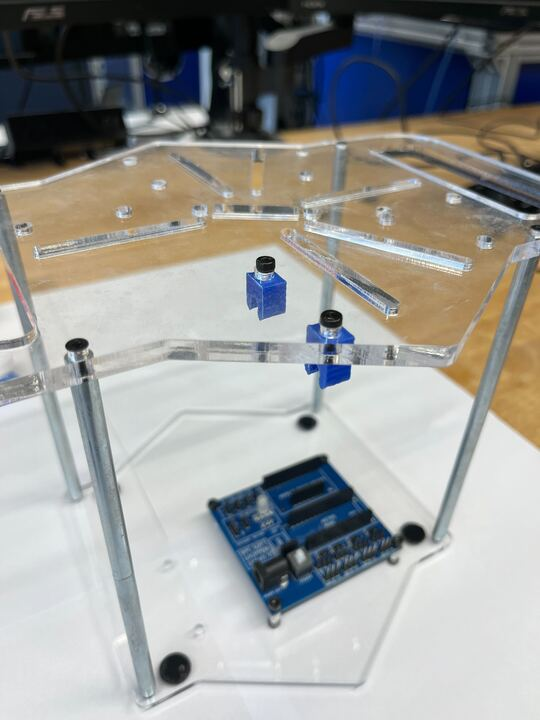
\includegraphics[width=0.5\linewidth]{PCBImages/StandoffClips/standoff_clips_6.jpg}
    \caption{Two Servo Clips attached to the proper place on the Top Plate}
    \label{fig:servo_clips_on_top_plate}
\end{figure}
\begin{figure}[H]
    \centering
    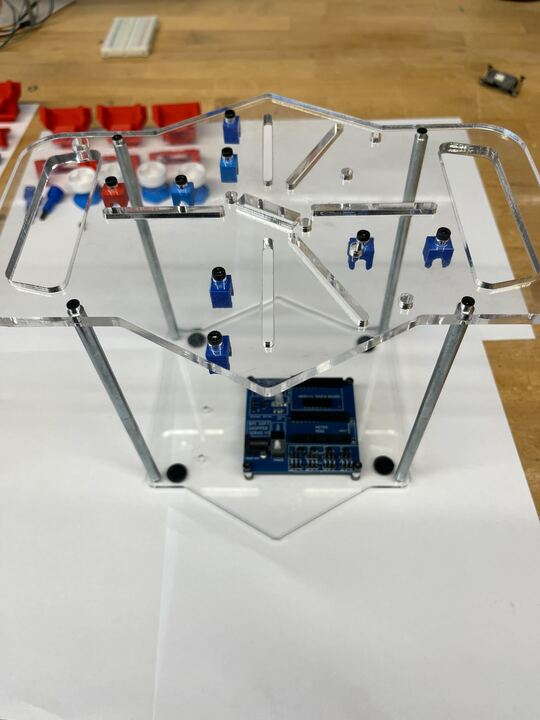
\includegraphics[width=0.5\linewidth]{PCBImages/StandoffClips/standoff_clips_7.jpg}
    \caption{All Servo Clips Attached}
    \label{fig:all_servo_clips_attached}
\end{figure}
\subsection{Placing the Servos on the Servo Standoff Clips}
\begin{figure}[H]
    \centering
    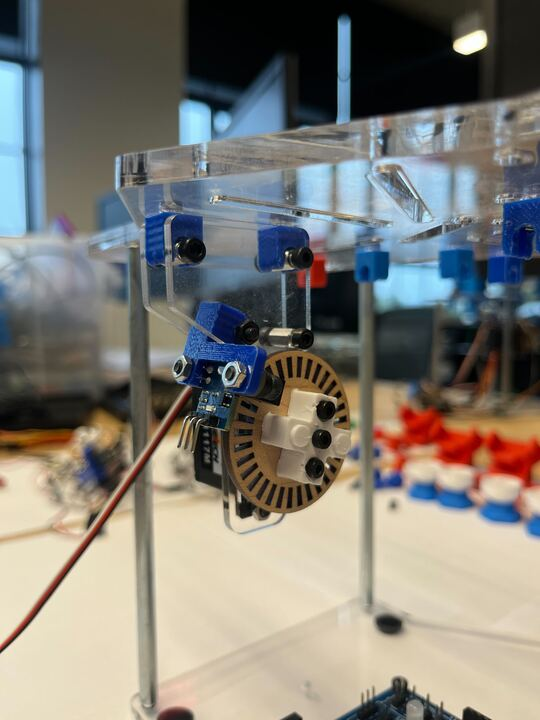
\includegraphics[width=0.5\linewidth]{PCBImages/AttachingServos/attaching_servos_1.jpg}
    \caption{Servo Clipped into the Servo Clips}
    \label{fig:servo_clipped_into_clips}
\end{figure}

\subsection{Connecting the Spool Base to the Servo}
\begin{figure}[H]
    \centering
    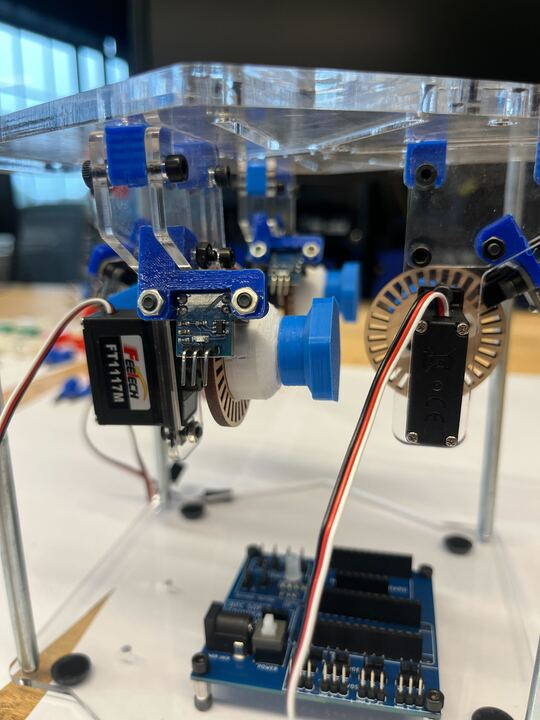
\includegraphics[width=0.5\linewidth]{PCBImages/AttachingServos/attaching_servos_2.jpg}
    \caption{The Spool magnetized to the Encoder Disk on the Servo Motor}
    \label{fig:spool_attached_to_servo}
\end{figure}

\section{Putting Together the PCB Board}

\subsection{Connecting the Encoders to the PCB}
\begin{figure}[H]
    \centering
    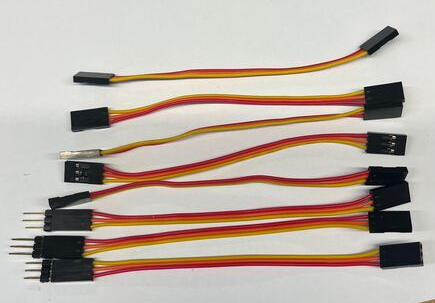
\includegraphics[width=0.5\linewidth]{PCBImages/EncoderWires/encoder_wires_1.png}
    \caption{Encoder Wires}
    \label{fig:enter-label}
\end{figure}

\begin{figure}[H]
    \centering
    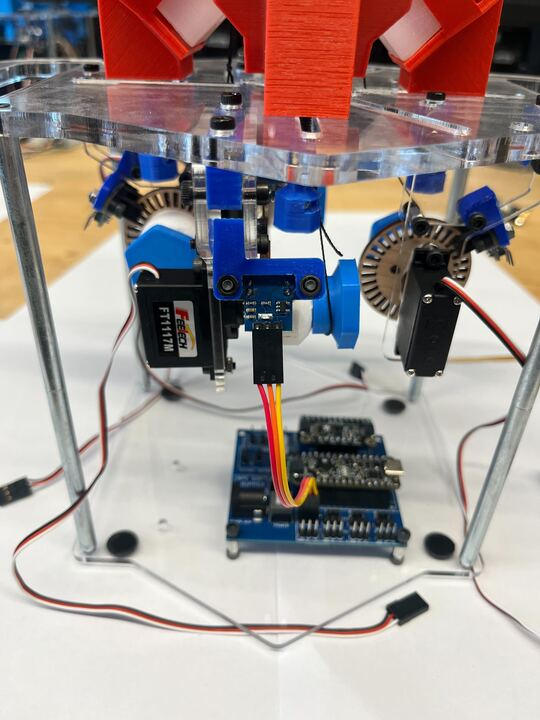
\includegraphics[width=0.5\linewidth]{PCBImages/EncoderWires/encoder_wires_2.jpg}
    \caption{An Encoder Wire attached to the Encoder Pins}
    \label{fig:enter-label}
\end{figure}

\begin{figure}[H]
    \centering
    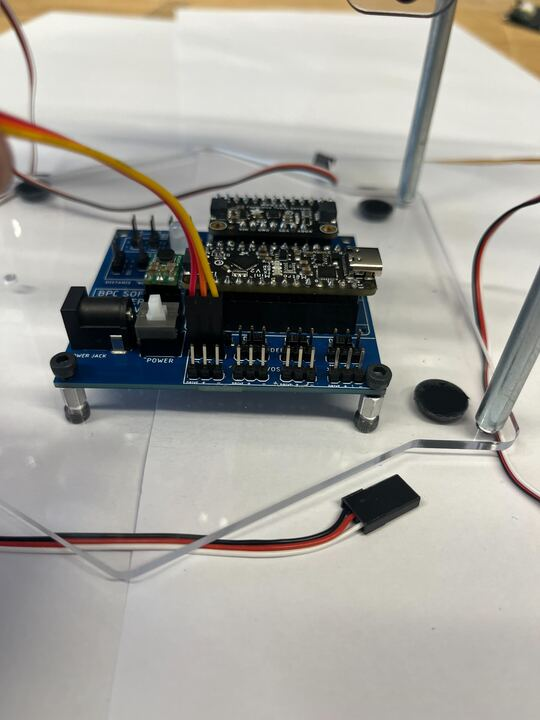
\includegraphics[width=0.5\linewidth]{PCBImages/EncoderWires/encoder_wires_3.jpg}
    \caption{Encoder Wire attached to Encoder Pins on the PCB Board}
    \label{fig:enter-label}
\end{figure}

\begin{figure}[H]
    \centering
    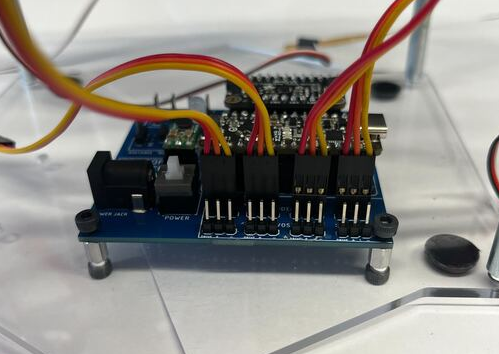
\includegraphics[width=0.5\linewidth]{PCBImages/EncoderWires/encoder_wires_4.png}
    \caption{All 4 Encoder Wires attached to the Encoder Pins on the PCB Board}
    \label{fig:enter-label}
\end{figure}



\subsection{Connecting the Servos to the PCB}

\begin{figure}[H]
    \centering
    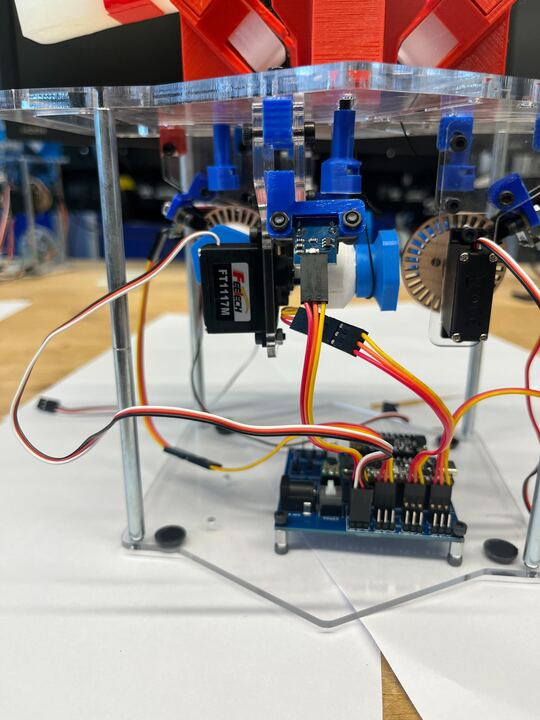
\includegraphics[width=0.5\linewidth]{PCBImages/ServoWires/servo_wires_1.jpg}
    \caption{Servo Motor Wires}
    \label{fig:enter-label}
\end{figure}

\begin{figure}[H]
    \centering
    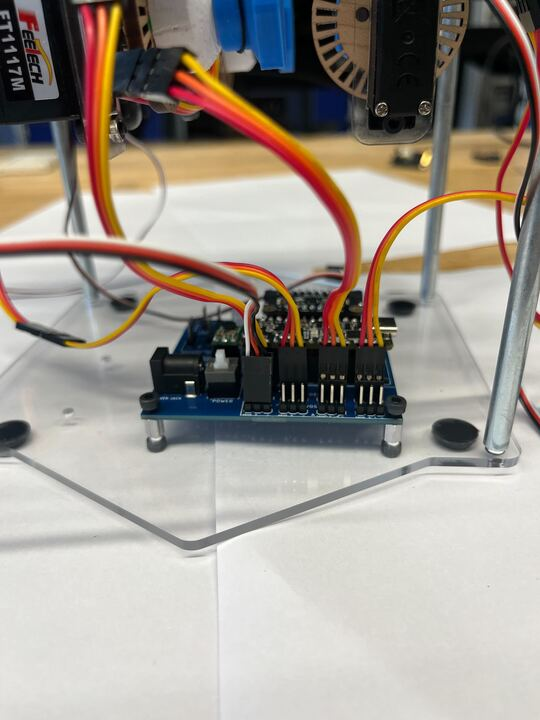
\includegraphics[width=0.5\linewidth]{PCBImages/ServoWires/servo_wires_2.jpg}
    \caption{Servo Motor Wires attached to Servo Pins on the PCB Board}
    \label{fig:enter-label}
\end{figure}

\begin{figure}[H]
    \centering
    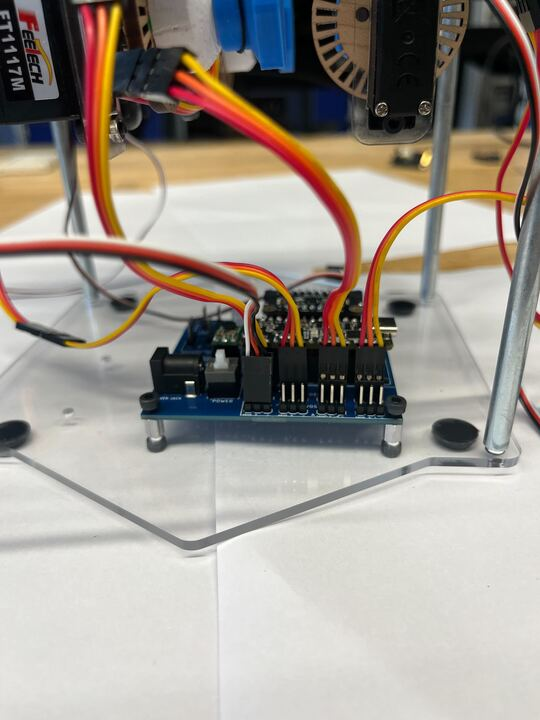
\includegraphics[width=0.5\linewidth]{PCBImages/ServoWires/servo_wires_2.jpg}
    \caption{All 4 Servo Wires attached to the Servo Pins on the PCB Board}
    \label{fig:enter-label}
\end{figure}



\subsection{Connecting the Ultrasonic Distance Sensor to the PCB}



we may want to put this to before we add the servos on, was kinda hard to attach them, also have to add 2 long screws, washers, and gold standoffs to piece list



\subsection{Connecting the Red Push Button to the PCB}

\begin{figure}[H]
    \centering
    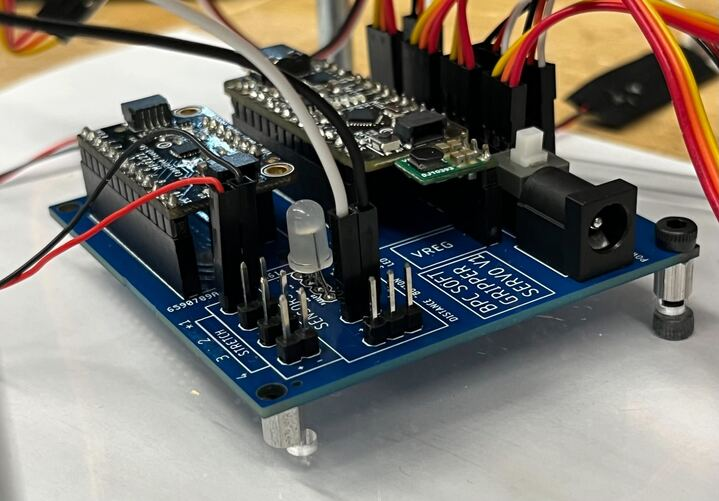
\includegraphics[width=0.5\linewidth]{PCBImages/RedButtonWiring/red_button_wiring_1.jpg}
    \caption{The Red Push Button Connected to the PCB Board}
    \label{fig:enter-label}
\end{figure}



\subsection{Connecting the Stretch Sensor(s) to the PCB}

\begin{figure}[H]
    \centering
    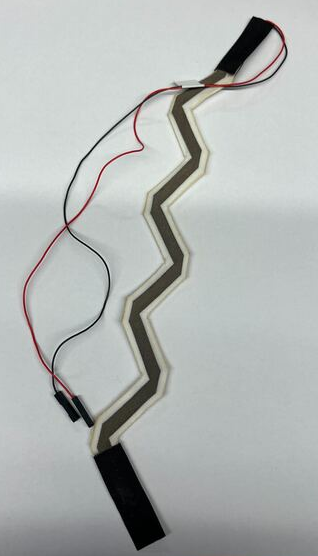
\includegraphics[width=0.5\linewidth]{PCBImages/StretchSensor/stretch_sensor_1.png}
    \caption{Stretch Sensor}
    \label{fig:enter-label}
\end{figure}

\begin{figure}[H]
    \centering
    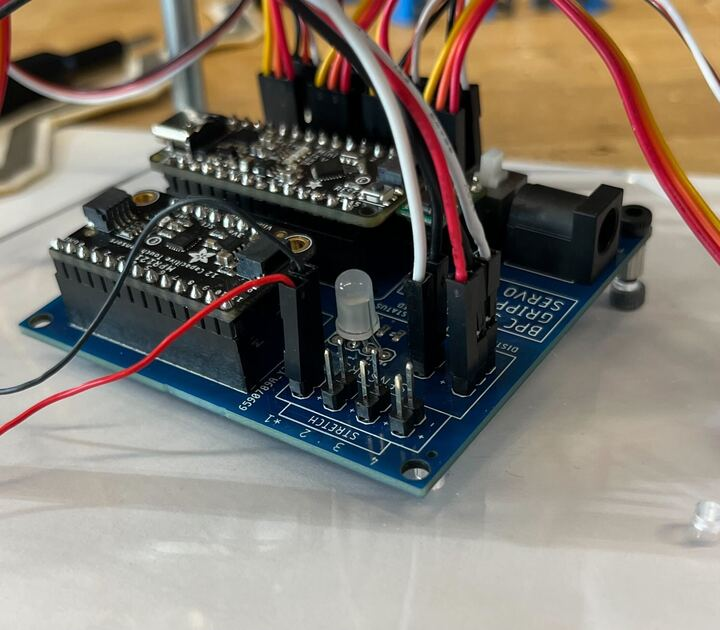
\includegraphics[width=0.5\linewidth]{PCBImages/StretchSensor/stretch_sensor_2.jpg}
    \caption{Stretch Sensor Wiring Connection}
    \label{fig:enter-label}
\end{figure}



\subsection{Placing the MPR121 on the PCB}
\begin{figure}[H]
    \centering
    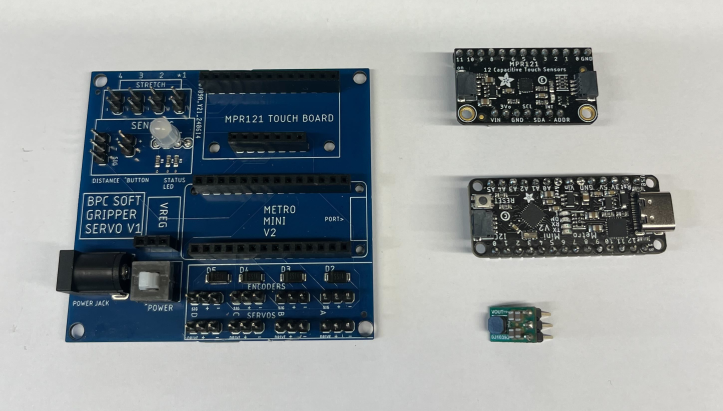
\includegraphics[width=0.5\linewidth]{PCBImages/PlacingPCBComponents/placing_pcb_components_2.png}
    \caption{The Base Plate}
    \label{fig:enter-label}
\end{figure}
\begin{figure}[H]
    \centering
    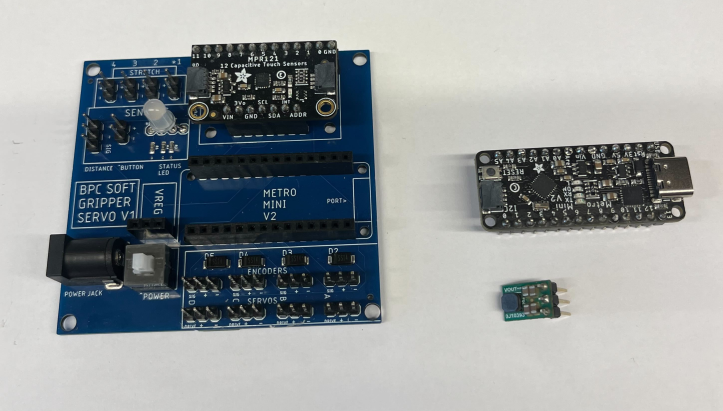
\includegraphics[width=0.5\linewidth]{PCBImages/PlacingPCBComponents/placing_pcb_components_1.png}
    \caption{Placing MPR121}
    \label{fig:enter-label}
\end{figure}

\subsection{Placing the Metro Mini V2 on the PCB}
\begin{figure}[H]
    \centering
    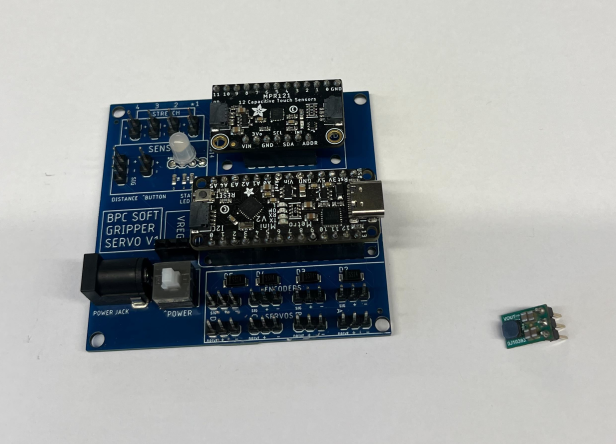
\includegraphics[width=0.5\linewidth]{PCBImages/PlacingPCBComponents/placing_pcb_components_3.png}
    \caption{Placing Metro Mini V2}
    \label{fig:enter-label}
\end{figure}




\subsection{Placing the Voltage Regulator on the PCB}
\begin{figure}[H]
    \centering
    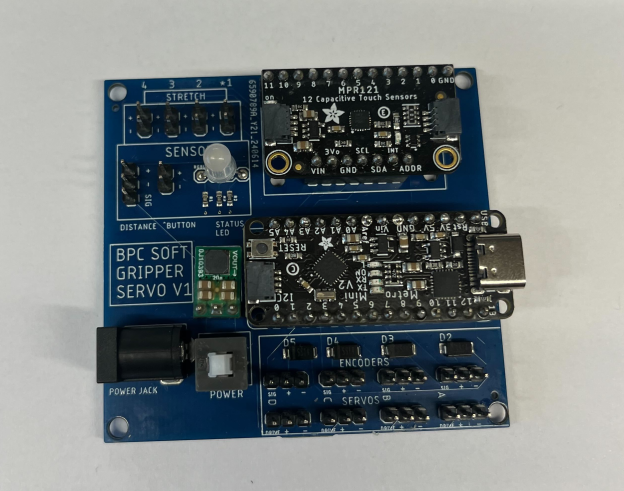
\includegraphics[width=0.5\linewidth]{PCBImages/PlacingPCBComponents/placing_pcb_components_4.png}
    \caption{Placing Voltage Regulator}
    \label{fig:enter-label}
\end{figure}



\section{Final Assembly}


\end{document}
